% Template for Cogsci submission with R Markdown

% Stuff changed from original Markdown PLOS Template
\documentclass[10pt, letterpaper]{article}

\usepackage{cogsci}
\usepackage{pslatex}
\usepackage{float}
\usepackage{caption}

% amsmath package, useful for mathematical formulas
\usepackage{amsmath}

% amssymb package, useful for mathematical symbols
\usepackage{amssymb}

% hyperref package, useful for hyperlinks
\usepackage{hyperref}

% graphicx package, useful for including eps and pdf graphics
% include graphics with the command \includegraphics
\usepackage{graphicx}

% Sweave(-like)
\usepackage{fancyvrb}
\DefineVerbatimEnvironment{Sinput}{Verbatim}{fontshape=sl}
\DefineVerbatimEnvironment{Soutput}{Verbatim}{}
\DefineVerbatimEnvironment{Scode}{Verbatim}{fontshape=sl}
\newenvironment{Schunk}{}{}
\DefineVerbatimEnvironment{Code}{Verbatim}{}
\DefineVerbatimEnvironment{CodeInput}{Verbatim}{fontshape=sl}
\DefineVerbatimEnvironment{CodeOutput}{Verbatim}{}
\newenvironment{CodeChunk}{}{}

% cite package, to clean up citations in the main text. Do not remove.
\usepackage{cite}

\usepackage{color}

% Use doublespacing - comment out for single spacing
%\usepackage{setspace}
%\doublespacing


% % Text layout
% \topmargin 0.0cm
% \oddsidemargin 0.5cm
% \evensidemargin 0.5cm
% \textwidth 16cm
% \textheight 21cm

\title{Preserved Structure Across Vector Space Representations}

\usepackage[utf8]{inputenc}
\usepackage[export]{adjustbox}

\author{{\large \bf Andrei Amatuni, Estelle He, Elika Bergelson} \\ \texttt{\{andrei.amatuni, estelle.he, elika.bergelson\}@duke.edu} \\ 417 Chapel Dr. Durham, NC 27708 USA \\ Department of Psychology and Neuroscience \\ Duke University}

\begin{document}

\maketitle

\begin{abstract}
Certain concepts, words, and images are intuitively more similar than
others (dog vs.~cat, dog vs.~spoon), though quantifying such similarity
is notoriously difficult. Indeed, this kind of computation is likely a
critical part of learning the category boundaries for words within a
given language. Here, we use a set of items (n= 27, e.g. `dog') that are
highly common in young infants' input, and use both image- and
word-based algorithms to independently compute similarity among these
items. We find three key results. First, the pair-wise item similarities
derived within image-space and word-space are correlated, suggesting
evidence of preserved structure among these extremely different
representational formats. Second, the closest `neighbors' for each item,
within each space, showed significant overlap (e.g.~both image- and
word-space found `egg' as a neighbor of `apple'). Third, items with the
most overlapping neighbors are later-learned by infants and toddlers. We
conclude that this approach, which does not rely on human ratings of
similarity, may nevertheless reflect stable within-class structure
across these two spaces. We speculate that such invariance, in turn,
might aid in lexical acquisition, by serving as an informative marker of
category boundaries.

\textbf{Keywords:}
vector space models; semantic similarity; word learning
\end{abstract}

\section{Introduction}\label{introduction}

Infants are presented with a challenge to carve the world into distinct
lexical entities in the process of learning their first language.
They're provided with little supervision while mapping a territory that
William James (1890) famously dubbed a ``great blooming, buzzing
confusion''. How they determine which aspects of the world to attend to
in service of this goal is an area of ongoing research and debate
(Mareschal \& Quinn, 2001). Relatedly, features of objects and their
environments are varyingly informative with regards to object
segmentation and category structure. Some researchers have suggested
that categorization is along fundamentally perceptual grounds and that
only later in development is conceptual knowledge incorporated into
these nascent perceptual categories (Quinn \& Eimas, 1997, 2000; Quinn,
Johnson, Mareschal, Rakison, \& Younger, 2000). Others suggest that
there are in fact two distinct processes at work, such that perceptual
categories are computed automatically by the sensory systems, while
conceptual categories are independently formed through conscious action
(Mandler, 2000). Träuble and Pauen (2007) provide evidence of functional
information (regarding the animacy of objects) influencing early
category judgements. Gelman and Markman (1986) explicitly set these two
sources of category cues against each other (i.e.~functional
vs.~perceptual), and find that preschoolers can override perceptual
overlap in reasoning about functional similarity, in natural kinds.

The degree to which conceptual and perceptual information are separable,
both in early learning, and in adult experts, is an important open
question. Any model which hopes to explain the mechanics of human
categorization must address how these potentially disparate
information-sources interface in mental representations, and to what
degree they interact. Indeed, evidence from human learners suggests they
integrate perceptual and linguistic information during categorization
and learning (\textbf{REFS e.g.~some of ref 12-19 in Waxman and Gelman
2009}). Here we take first steps in a deliberately different approach.
We separate computations over images and words, and then compare the
overlap in the similarity among items that these systems deduce. Using a
set of highly familiar and common words and concepts from a large infant
corpus, we compare the output of an image-based similarity analysis, and
a word co-occurrence similarity analysis for these same items. We use
algorithms that learn feature representations without hand engineering,
purely as a byproduct of their particular (and separate) training
objectives (e.g.~natural language processing or object recognition in
images). Comparing the representations these algorithms learn, we gain a
window into the structure of visual and semantic forms.

The terminlogy in this area of research can be challenging. Delineating
the differences between words, concepts, and categories in the abstract,
and the processes which underly identifying, understanding, or comparing
particular instances of them in the world is not trivial. For present
purposes, we stick to concrete, `basic level' nouns that are
early-acquired, since our underlying question concerns how such words
are learned. We assume that nouns refer to concepts, which have
categorical boundaries (such that cats are not in the `dog' category),
while acknowledging that multiple nouns can refer to a given concept,
and different concepts can be called to mind by a given word. We further
assume that specific instances of words in natural language production,
and specific images of the concept a word picks out are both used by
learners to inform their understanding of what the word means, and what
the category boundaries of the concept are. Hereafter we use the term
`item' to refer to the words/concepts we examine.

Intuitively, word similarity and image similarity are likely to overlap
to some degree, since they describe the same underlying entity. Here we
explore whether the similarity spaces generated by two disparate
algorithms give rise to \emph{similar} similarities among our
high-frequency items. If they do, it lends credence to the notion of an
underlying invariance across representational formats that is capturable
by these models. We further examine whether the same ``neighboring''
items are picked out within these two spaces. One might imagine that the
properties that render images similar and words similar are different
enough that the overlap will be minimal; in contrast, high overlap would
again suggest a true invariance being captured by both word- and
image-tokens, as measured here. Finally, we examine whether having more
neighbors within word- and image-space influences early learning. Given
that similarity makes word-learning and category-learning more difficult
(Rosch \& Lloyd, 1978; Stager \& Werker, 1997), we hypothesize that
items with more neighbors will be later-learned (or put otherwise, known
by fewer children of a given age.)

\section{Methods}\label{methods}

\subsection{Items}\label{items}

The 27 items analyzed here were selected due to their high frequency in
infants' early visual and linguistic input, aggregated as part of the
SEEDLingS project, which gathered longitudinal audio and video data of
infants' home environments from 6-17 months (E. Bergelson, 2016a,
2016b). We describe this larger study in brief, simply to relay how the
items we analyze were chosen; the details of this larger study are not
critical to the present work. In the larger study, 44 infants were
tested every other month (from 6-18 months) on common nouns, using a
looking-while-listening eyetracking design in which two images are shown
on a screen, and one is named. The words for these experiments were
chosen by dint of being high frequency or well known across infants in
other samples, e.g.~the Brent Corpus and WordBank (Brent \& Siskind,
2001; Frank, Braginsky, Yurovsky, \& Marchman, 2017), or by being one of
the top 10 concrete nouns heard in each infant's own home audio and
video recordings in the preceding two months.

The images displayed when these words were tested were chosen from a
library of prototypical images of a given word (e.g.~dog), along with
images of infants' own versions of the items, as seen in their home
videos (e.g.~a given infant's cat, specific bottle, etc.). To enter the
current analysis, images had to occur 9 or more times in this image
library of high frequency concrete nouns derived from 264 eyetracking
sessions (image counts: mean=18.85, SD=10.89). These words were heard
extremely often over the 528 daylong audio-recordings and 528 hour-long
video recordings of these 44 infants (mean=2034.85, SD=1540.22). Thus,
the words and images used here provide an ecologically-valid item-set
for present modeling purposes.

The images of the 27 items used to derive average category image-vectors
were all 960x960 pixel photos of a single object on a gray background.
All items correspond to words found on WordBank (Frank et al., 2017), a
compilation of the MacArthur-Bates Communicative Development Inventory,
which we use as a proxy for age of acquisition below (Dale \& Fenson,
1996).

\subsection{Vector Representations}\label{vector-representations}

We generate two sets of vector representations for a common set of
early-learned items. The first set of vectors are taken from a
pretrained set of GloVe representations (Pennington, Socher, \& Manning,
2014), a modern distributional semantic vector space model. The second
set is taken from the final layer activations of a pretrained image
recognition model, Google's Inception V3 convolutional neural network
(Szegedy, Vanhoucke, Ioffe, Shlens, \& Wojna, 2016). Both of these
representations are generally referred to as ``embeddings''. They map
objects from one medium (e.g.~images or words) into a metric space where
distances between points can be computed and function as a measure of
similarity between objects.

\subsubsection{Word Vectors}\label{word-vectors}

In the case of our word vectors, the GloVe algorithm instantiates the
distributional hypothesis, which proposes that words which co-occur with
each other share similar meaning (Firth, 1957; Harris, 1954). Thus, by
capturing the covariance of tokens in large text corpora, we can capture
aspects of their semantic structure. We use the set of vectors
pretrained by the GloVe authors on the Common Crawl corpus with 42
billion tokens, resulting in 300 dimensional vectors for 1.9 million
unique words\footnote{\url{https://nlp.stanford.edu/projects/glove/}}.
Such vectors have shown promise in modeling early semantic networks
(Amatuni \& Bergelson, 2017). Thus, in word vector space (hereafter
word-space), each of our 27 items is represented as a 300-dimensional
vector, with each word assigned a unique point in a common vector space.
\footnote{While the Common Crawl corpus is best-suited to our goal of modelling 'how words behave' writ large, we also conducted the analyses below with vectors trained on the North American English CHILDES corpora (MacWhinney, 2000), which is $\sim$4000x smaller. We observe the same qualitative patterns with both corpora.}

\subsubsection{Image Vectors}\label{image-vectors}

The image embeddings are taken from the final layer of activations in a
convolutional neural network, whose objective function tunes network
parameters in service of object recognition, computing loss in reference
to a set of labeled training images (Russakovsky et al., 2015). These
tuned parameters determine the value of our vectors, operating over and
transforming our input image signal as it passes through the network.
The final layer of this network encodes the most abstract and integrated
visual features, serving as the basis for classification into 1000
different classes.

Unlike for the word vectors we use, different images containing the same
type of item will have varying vector representations after passing
through the layers of a neural network. This presents a problem in
comparing the two forms of representation. We must first define the most
prototypical (or average) image vector for any given category of object,
which will generate our 2048-dimensional representation for each of the
27 items, in image vector space (hereafter image-space).

Given a set of images \(S_c\) containing objects belonging to a single
category \(c\) (e.g.~cat, dog, chair), we define our prototypical vector
\(\hat{x}_c\) of \(S_c\) as the generalized median within a
representational space \(U\). This is the vector with minimal sum of
distances between it and all the other members of set \(S_c\) in \(U\).
If \(x\) and \(y\) are vectors in space \(U\), products of images in
\(S_c\) being passed through a neural network, then

\[
 \hat{x}_c = \operatorname*{arg\,min}_{x\in U} \sum_{y\in U} d(x, y)
\] We define our \(d(x, y)\) to be the cosine similarity measure:

\[
d(x, y) = 1 - \frac{x\cdot y}{\|x\|\|y\|}
\]

Our \(d(x, y)\) is not a metric in the strict sense, but is less
susceptible to differences in \(L^2\) norm influencing our measure of
similarity, unlike Euclidean distance. Thus in principle, cosine
similarity corrects for frequency effects in training data. All code
used for generating these vectors and for the subsequent analysis can be
found on
Github\footnote{\url{https://github.com/BergelsonLab/preserved_structure}}.

\subsection{Comparing spaces}\label{comparing-spaces}

Having computed our two sets of vectors (i.e.~those from word-space and
those from image-space), we can compare all the pairwise distances
between objects, both within a single space and across the two. When
comparing across the two spaces, a correlation in pairwise distances
implies that inter-object distances have been conserved. For example, if
``dog'' and ``cat'' are close together in word space and mutually far
apart from ``chair'' and ``table'' in that same space, maintaining this
relationship for all pairwise distances in the \textit{other} vector
space means that the global inter-object structure is preserved across
this mapping, despite being in radically different spaces, both in terms
of dimensionality (300 for words, and 2048 for images in our case) and
by virtue of using completely different algorithms and inputs to
establish the vector representations for objects. So while their
absolute locations might have been radically transformed, this
correlation (and related computations) would be a measure of the
\textit{degree of invariance} in their positioning relative to each
other.

\section{Results}\label{results}

To test whether image- and word-based similarity converged for this set
of 27 items, we conducted several analyses. First, we tested whether the
pairwise cosine distances for all items in word-space correlated with
those same pairwise distances in the image-space (see Figure
\ref{fig:pairwise-corr}). Indeed, we find a significant correlation
among the 351 pairs of distances (\(R = 0.30\), \(p < 1.5e-08\)).
\footnote{since distances are identical for cat-dog and dog-cat, and since we omit an item's distance to itself (0), there are (27*27-27)/2) pairs of distances. For simplicty, we report Pearson's R and plot a linear fit on Figure 1, but note that non-parametric correlations (e.g. Spearman's $\rho$) reveal the same pattern.}

Next, we examined the degree to which our set of 27 words shared
overlapping `neighbors' in the two vector spaces (see Table
\ref{tbl:overlap-table}). We defined neighbor by first determining the
mean similarity distance between each item and the 26 other items. Any
items whose distance to this target had a zscore of less than -1 was
considered a neighbor. Within word-space, items had on average 3.3
neighbors (SD=1.27 , R=1-5). Within image-space, items had 2.51
neighbors (SD=1.6, R=0-6).

We next tested whether both spaces picked out overlapping neighbors
(e.g.~whether the neighbor of `cat' in image-space overlapped with the
neighbors of `cat' in word-space, see Table \ref{tbl:overlap-table}).
The majority of items have at least 1 neighbor which is shared across
representational spaces. To quantify this overlap, we computed `overlap'
ratios, which measured how many of the neighbors overlapped, divided by
how many neighbors there were. Overlap was significantly greater than 0
\textbf{(Mean(SD) Overlap XX, p\textless{} XX} by Wilcoxon test). This
complements the correlational analysis, showing not just that the
distances for any given pair tended to have similar values in
image-space and word-space, but that the \emph{most} similar
words/images (i.e.~each item's neighbors) were also consistent across
these spaces.

\section{Connecting with
Learnability}\label{connecting-with-learnability}

While some degree of convergence across image and word spaces is to be
expected given that these are two different manifestations of the same
underlying concept/word/item, we next queried whether this invariance
related to learnability. We hypothesized that words with more
overlapping neighbors would be harder for children to learn, since both
the visual and linguistic spaces they occur in are more `cluttered.' To
test this, we looked at the relative rates of acquisition of our 27
items in WordBank (Frank et al., 2017), using the 6945 children's data
from English. Since we did not have clear predictions about specific
ages, or of tradeoffs between comprehension and production, we used
both. That is, we used comprehension norms (from MCDI-Words and
Gestures, averaging over 8-18 months) and production norms (from
MCDI-Words and Sentences, averaging over 16-30 months).

We found that the number of overlapping neighbors a given word had was
negatively correlated with the proportion of children who were reported
to understand the word (R=-0.48, p \textless{} 0.01) and produce the
word (R=-0.46, p \textless{} 0.02); see Figure
\ref{fig:overlap-aoa-graphs}. That is, words with more overlapping
neighbors are later-learned (or put otherwise, known but fewer children)
than words with fewer overlapping neighbors. To test whether this was
specific to overlap, we examined the number of image-only and word-only
neighbors (see Table \ref{tbl:overlap-table})); these measures did not
correlate with word knowledge (all p\textgreater{}.05).

\begin{CodeChunk}
\begin{figure}[tb]
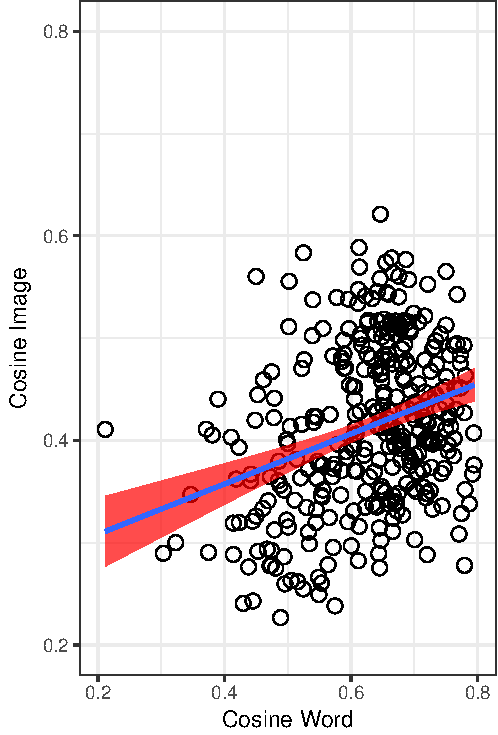
\includegraphics{figs/pairwise-corr-1} \caption[Relative cosine distance between points in word embedding space (x-axis) and image embedding space (y-axis), for every item pair]{Relative cosine distance between points in word embedding space (x-axis) and image embedding space (y-axis), for every item pair. Fitted line reflects linear fit with SE;the correlation is significant ($R = 0.30$, $p < 1.5e-08$).}\label{fig:pairwise-corr}
\end{figure}
\end{CodeChunk}

\begin{table}
\centering
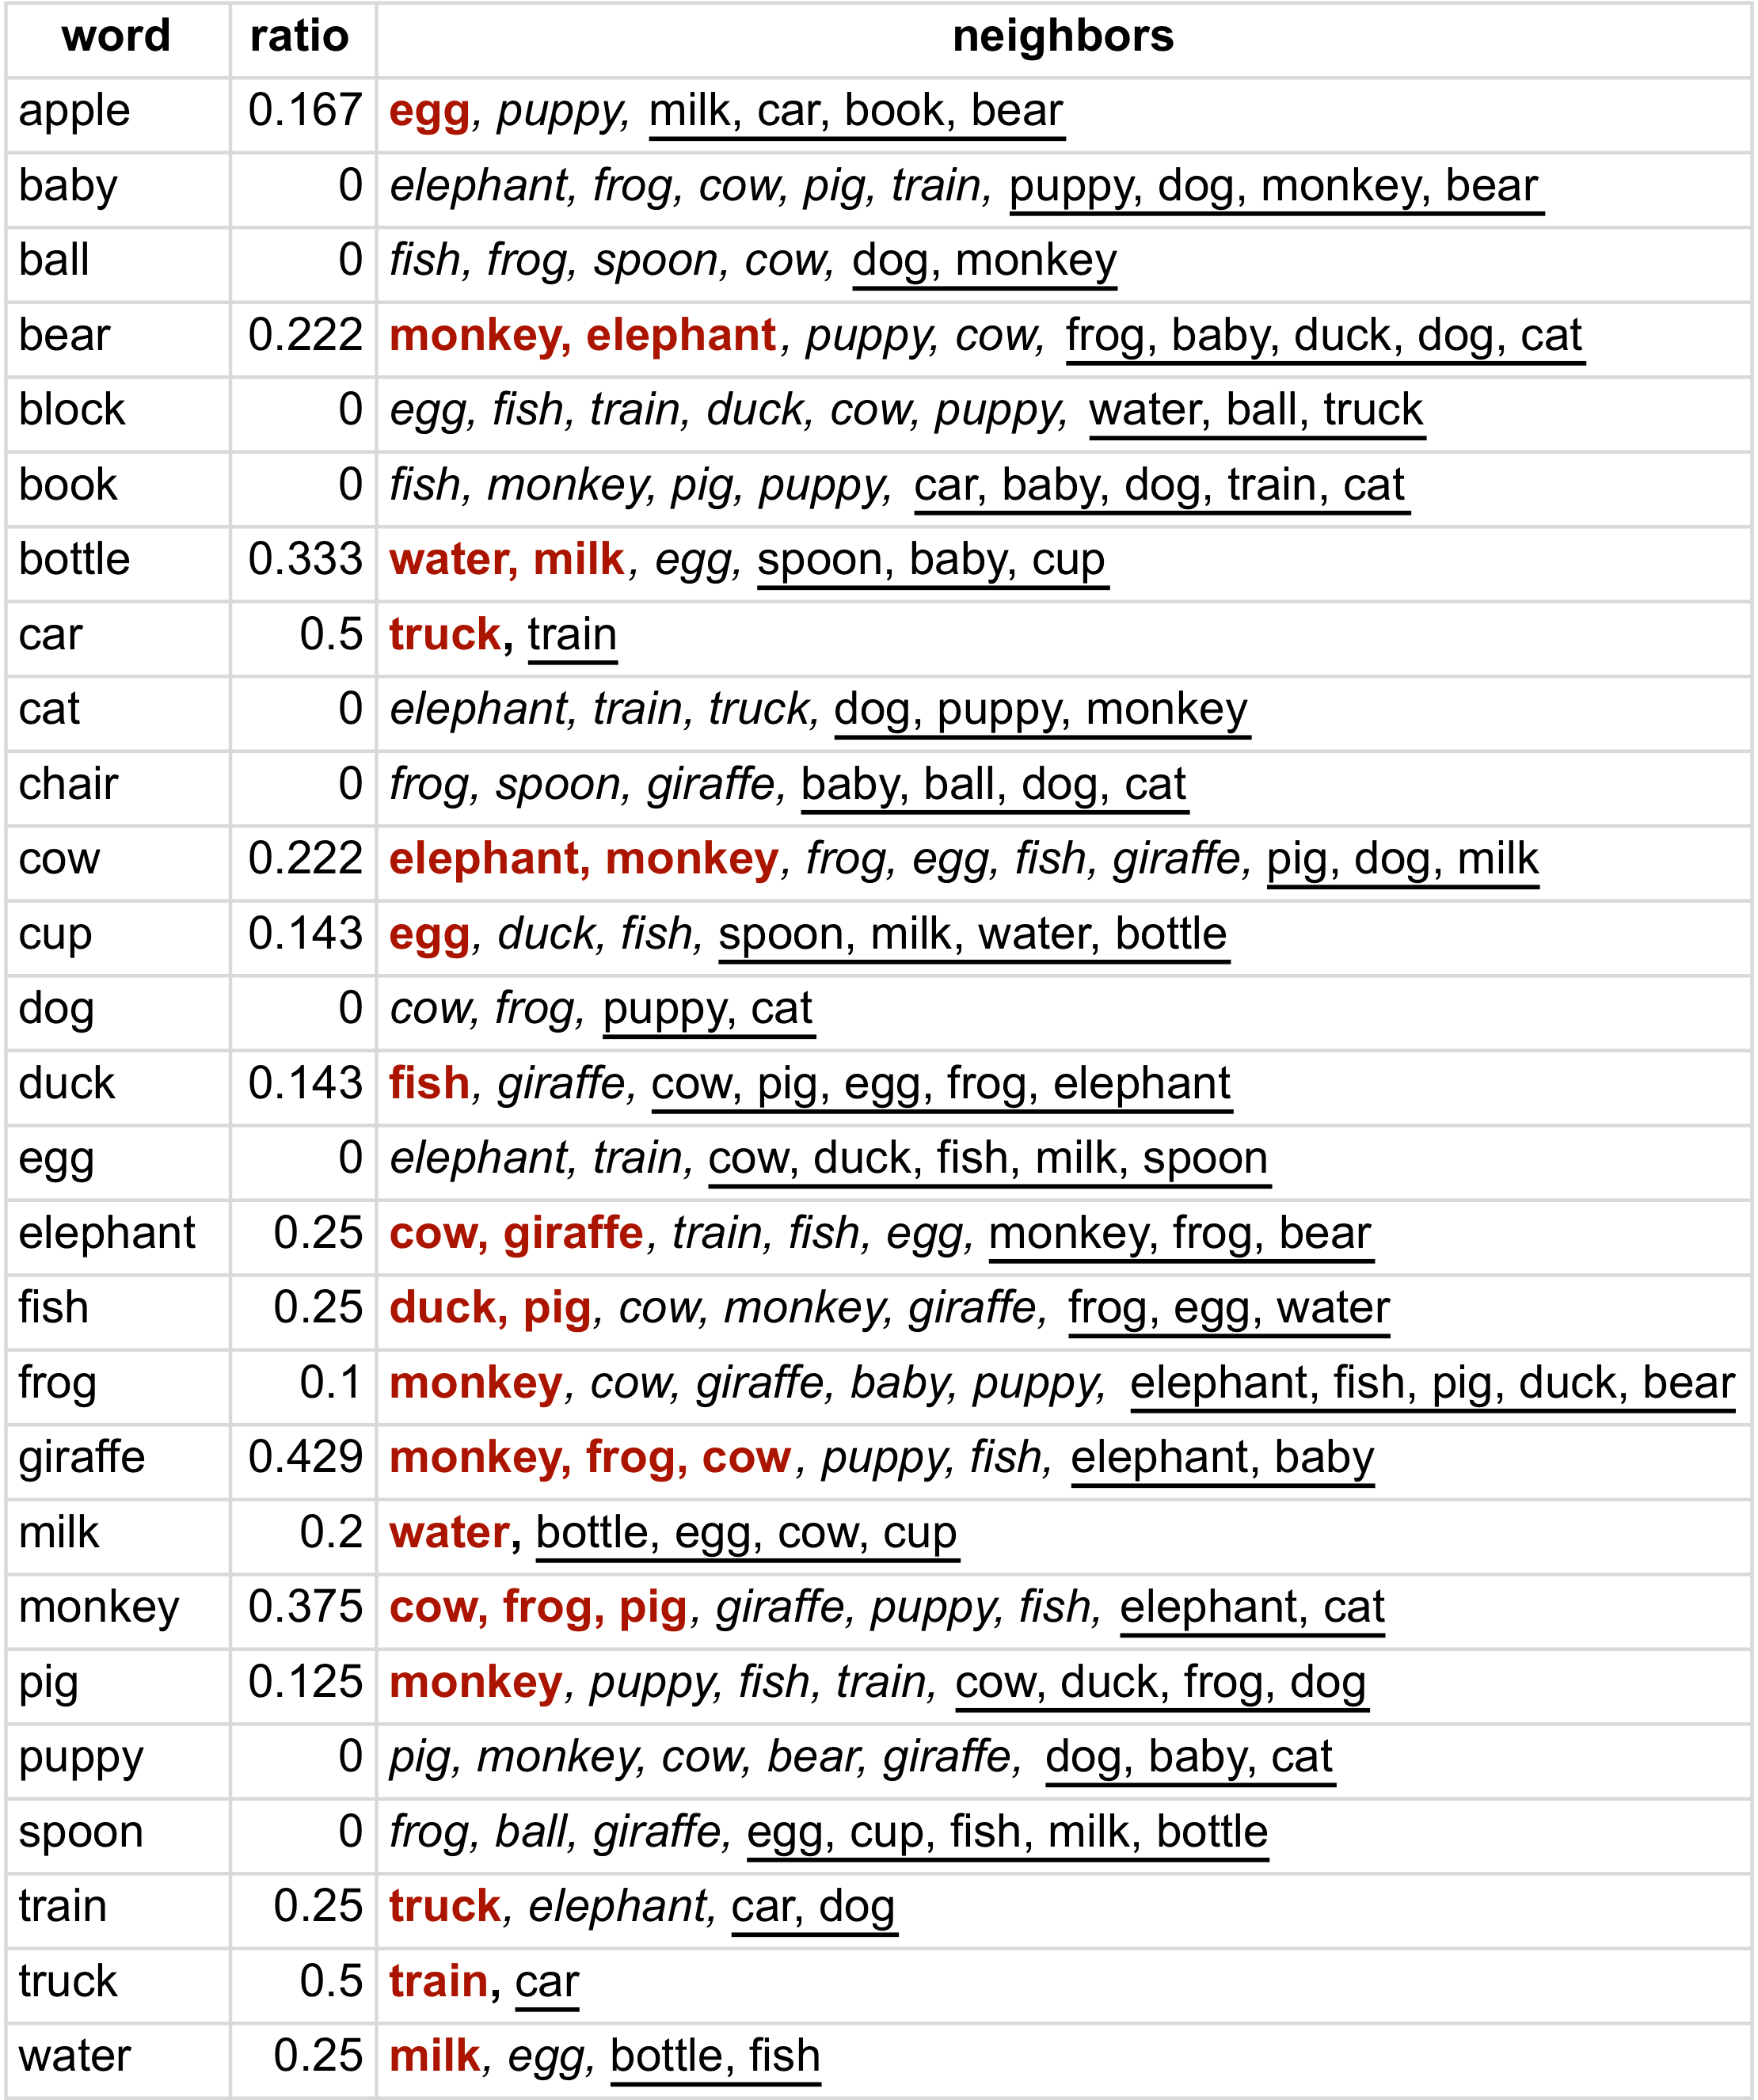
\includegraphics[max size={0.9\columnwidth}{0.7\textheight}]{data/overlap_table_formatted2.png}
\caption{Neighbors in image- and word-space. Neighbors in bold and red are shared between spaces; italicised words are image-neighbors only, underlined words are word-neighbors only. Overlap ratio reflects shared neighbors over total neighbors. See text for details.}
\label{tbl:overlap-table}
\end{table}

\begin{CodeChunk}
\begin{figure}[tb]
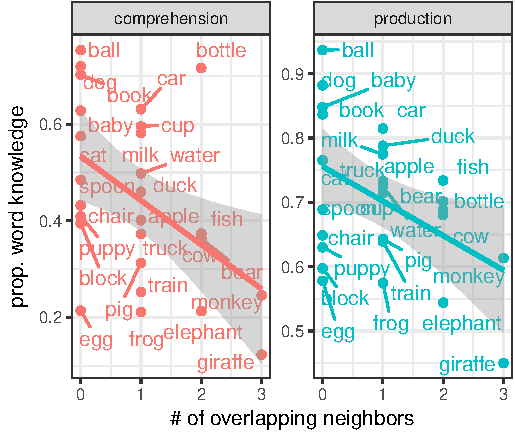
\includegraphics{figs/overlap-aoa-graphs-1} \caption[Proportion of children in WordBank reported to understand (left, averaged over 8-18 months) or produce (right, averaged over 16-30 months) the 27 items, as a function of how many overlapping neighbors (i.e]{Proportion of children in WordBank reported to understand (left, averaged over 8-18 months) or produce (right, averaged over 16-30 months) the 27 items, as a function of how many overlapping neighbors (i.e. in both image- and word-space) they have. Line indicates linear fit with SE confidence band.}\label{fig:overlap-aoa-graphs}
\end{figure}
\end{CodeChunk}

\section{Discussion}\label{discussion}

The results above revealed a significant correspondence between
representations learned by two different algorithms operating over
inputs in two fundamentally different encoding formats (i.e.~visual and
linguistic). We find that not only are the relative distances among
these 27 common, early-learned items correlated across word- and
image-space, but that even at the item-level, the `closest' words in
both spaces overlap as well. What is most noteworthy here is that the
only immediate common ground between these representations are the real
life concepts they both aim to model. This is particularly notable given
the enormous dimensionality of our feature spaces, and the fact that
these algorithms are placed under no pressure to find homologous
representations.

The notion that we can make inferences about one aspect of an object
given another aspect is not surprising or controversial. Rather than
considering multiple dimensions of a word or concept at once, as real
learners must, here we show that even with the experiences parcelled out
separately into visual and linguistic spaces, what counts as `similar'
is conserved to some degree.

Through what metrics can a learning algorithm, or indeed a human,
establish gradations of likeness? Are these necessarily the same metrics
which form the basis of category boundaries? These are fundamental
questions which have enjoyed a long history in the field (Edelman, 1998;
Hahn, Chater, \& Richardson, 2003; Kemp, Bernstein, \& Tenenbaum, 2005;
Shepard \& Chipman, 1970; Tversky, 1977). While our current work is not
sufficient to support a specific mechanism responsible for the observed
regularity, it might be indicative of the special role of invariance,
given that the unifying thread between our algorithms and inputs are the
common objects they represent. Underneath the diversity of visual
statistics and token distributions lie stable entities in the world
which, by virtue of their invariant actuality, give rise to regularity
across measurements at different vantage points (i.e.~modalities), an
idea dating back to Helmholtz (1878). Recent work examining the
mechanics of generalization in deep neural networks lends modern
information theoretic support to this notion (Achille \& Soatto, 2017;
Shwartz-Ziv \& Tishby, 2017). That said, many things that `go together'
are not visually similar, but rather have hiearchical, functional, or
associative relations (e.g.~carrot/vegetable, skateboard/board,
carrot/bunny, respetively). Indeed, while concrete nouns are an
appropriate target for these current analyses, given their demonstrably
early age of acquisition (Dale \& Fenson, 1996), further work with more
abstract words (nouns and beyond) would likely be fruitful.

In principle, one would expect that words with greater invariance across
different representational dimensions would be learned earlier. I.e.
visibly round objects appear in sentences about rolling, and these sorts
of correlated cue have been shown to aid the child learner
{[}yoshida2005linguistic{]}. Our WordBank-based analysis speaks to this,
highlighting that when the space is cluttered along both visual and
linguistic dimensions, learning is slowed. Indeed, such an account is in
keeping with infant and toddler research that finds that for displays of
semantically-similar items, word comprehension is reduced (Arias-Trejo
\& Plunkett, 2010; E. Bergelson \& Aslin, 2017).

The results here provide in-principle proof that vector space models of
words and images can fruitfully be combined and linked to early language
and concept learning. Indeed, our approach could readily be extended to
examine properties known to be relevant to early learning like animacy,
shape, and color {[}e.g., frank2009development;landau1992syntactic{]}.
Indeed, in an exploratory analyses with these items, we find that
splitting item-pairs into animate, inanimate, and mixed categories
suggests that the image- and word-based correlation is particularly
strong for the inanimate items, though with only 27 items, further
conclusions are as-yet unwarranted. However, one can imagine that in a
larger database of childrens' visual and linguistic experiences, tests
of overlapping similarity may provide fruitful leverage for predicting
age of acquisition across the early vocabulary.

\section{Conclusion}\label{conclusion}

We find evidence of links between visual and semantic features learned
by two distinct machine learning algorithms which operate over
drastically different inputs, and are trained in the service of
seemingly unrelated ends. These links suggest conserved structure
between these two separable sources of information (i.e.~visual and
linguistic). Indeed, it seems that not only do these algorithms converge
on which words are `closer' in similarity, within a group of oft-heard
and seen concrete nouns, but human learners too are sensitive to these
overlapping cross-word relationships. The process that created the word-
and image-spaces we examine here is certainly not meant to be
cognitively plausible. Nevertheless, our results suggest that this
vector-space approach can be tied to language acquistion, and provides
promising new avenues for uncovering cross-representational influences
on early word and concept learning.

\section{Acknowledgements}\label{acknowledgements}

We thank the SEEDLingS team, and NIH DP5-OD019812.

\section{References}\label{references}

(MacWhinney, 2000)

\setlength{\parindent}{-0.1in} \setlength{\leftskip}{0.125in} \noindent

\hypertarget{refs}{}
\hypertarget{ref-achille2017emergence}{}
Achille, A., \& Soatto, S. (2017). On the emergence of invariance and
disentangling in deep representations. \emph{arXiv Preprint
arXiv:1706.01350}.

\hypertarget{ref-amatuni2017semantic}{}
Amatuni, A., \& Bergelson. (2017). Semantic networks generated from
early linguistic input. In \emph{Proceedings of the 39th annual
conference of the cognitive science society} (pp. 1538--1543).

\hypertarget{ref-arias2010effects}{}
Arias-Trejo, N., \& Plunkett, K. (2010). The effects of perceptual
similarity and category membership on early word-referent
identification. \emph{Journal of Experimental Child Psychology},
\emph{105}(1-2), 63--80.

\hypertarget{ref-bergelson2016seedlings}{}
Bergelson, E. (2016a). Bergelson seedlings homebank corpus.
\url{http://doi.org/10.21415/T5PK6D}

\hypertarget{ref-bergelson2016seedlingsdatabrary}{}
Bergelson, E. (2016b). SEEDLingS corpus. Retrieved January 26, 2018,
from \url{https://nyu.databrary.org/volume/228}

\hypertarget{ref-bergelson2017nature}{}
Bergelson, E., \& Aslin, R. N. (2017). Nature and origins of the lexicon
in 6-mo-olds. \emph{Proceedings of the National Academy of Sciences},
\emph{114}(49), 12916--12921.

\hypertarget{ref-brent2001role}{}
Brent, M. R., \& Siskind, J. M. (2001). The role of exposure to isolated
words in early vocabulary development. \emph{Cognition}, \emph{81}(2),
B33--B44.

\hypertarget{ref-dale1996lexical}{}
Dale, P. S., \& Fenson, L. (1996). Lexical development norms for young
children. \emph{Behavior Research Methods, Instruments, \& Computers},
\emph{28}(1), 125--127.

\hypertarget{ref-edelman1998representation}{}
Edelman, S. (1998). Representation is representation of similarities.
\emph{Behavioral and Brain Sciences}, \emph{21}(4), 449--467.

\hypertarget{ref-firth1957synopsis}{}
Firth, J. R. (1957). A synopsis of linguistic theory, 1930-1955.
\emph{Studies in Linguistic Analysis}.

\hypertarget{ref-frank2017wordbank}{}
Frank, M. C., Braginsky, M., Yurovsky, D., \& Marchman, V. A. (2017).
Wordbank: An open repository for developmental vocabulary data.
\emph{Journal of Child Language}, \emph{44}(3), 677--694.

\hypertarget{ref-gelman1986categories}{}
Gelman, S. A., \& Markman, E. M. (1986). Categories and induction in
young children. \emph{Cognition}, \emph{23}(3), 183--209.

\hypertarget{ref-hahn2003similarity}{}
Hahn, U., Chater, N., \& Richardson, L. B. (2003). Similarity as
transformation. \emph{Cognition}, \emph{87}(1), 1--32.

\hypertarget{ref-harris1954distributional}{}
Harris, Z. S. (1954). Distributional structure. \emph{Word},
\emph{10}(2-3), 146--162.

\hypertarget{ref-helmholtz1878facts}{}
Helmholtz, H. (1878). The facts of perception. \emph{Selected Writings
of Hermann Helmholtz}, 1--15.

\hypertarget{ref-james2013principles}{}
James, W. (1890). \emph{The principles of psychology}. Henry Holt;
Company.

\hypertarget{ref-kemp2005generative}{}
Kemp, C., Bernstein, A., \& Tenenbaum, J. B. (2005). A generative theory
of similarity. In \emph{Proceedings of the 27th annual conference of the
cognitive science society} (pp. 1132--1137).

\hypertarget{ref-macwhinney2000childes}{}
MacWhinney, B. (2000). \emph{The childes project: The database} (Vol.
2). Psychology Press.

\hypertarget{ref-mandler2000perceptual}{}
Mandler, J. M. (2000). Perceptual and conceptual processes in infancy.
\emph{Journal of Cognition and Development}, \emph{1}(1), 3--36.

\hypertarget{ref-mareschal2001categorization}{}
Mareschal, D., \& Quinn, P. C. (2001). Categorization in infancy.
\emph{Trends in Cognitive Sciences}, \emph{5}(10), 443--450.

\hypertarget{ref-pennington2014glove}{}
Pennington, J., Socher, R., \& Manning, C. (2014). Glove: Global vectors
for word representation. In \emph{Proceedings of the 2014 conference on
empirical methods in natural language processing (emnlp)} (pp.
1532--1543).

\hypertarget{ref-quinn1997reexamination}{}
Quinn, P. C., \& Eimas, P. D. (1997). A reexamination of the
perceptual-to-conceptual shift in mental representations. \emph{Review
of General Psychology}, \emph{1}(3), 271.

\hypertarget{ref-quinn2000emergence}{}
Quinn, P. C., \& Eimas, P. D. (2000). The emergence of category
representations during infancy: Are separate perceptual and conceptual
processes required? \emph{Journal of Cognition and Development},
\emph{1}(1), 55--61.

\hypertarget{ref-quinn2000understanding}{}
Quinn, P. C., Johnson, M. H., Mareschal, D., Rakison, D. H., \& Younger,
B. A. (2000). Understanding early categorization: One process or two?
\emph{Infancy}, \emph{1}(1), 111--122.

\hypertarget{ref-rosch1978cognition}{}
Rosch, E., \& Lloyd, B. B. (1978). Cognition and categorization.

\hypertarget{ref-ILSVRC15}{}
Russakovsky, O., Deng, J., Su, H., Krause, J., Satheesh, S., Ma, S.,
\ldots{} Fei-Fei, L. (2015). ImageNet Large Scale Visual Recognition
Challenge. \emph{International Journal of Computer Vision (IJCV)},
\emph{115}(3), 211--252. \url{http://doi.org/10.1007/s11263-015-0816-y}

\hypertarget{ref-shepard1970second}{}
Shepard, R. N., \& Chipman, S. (1970). Second-order isomorphism of
internal representations: Shapes of states. \emph{Cognitive Psychology},
\emph{1}(1), 1--17.

\hypertarget{ref-shwartz2017opening}{}
Shwartz-Ziv, R., \& Tishby, N. (2017). Opening the black box of deep
neural networks via information. \emph{arXiv Preprint arXiv:1703.00810}.

\hypertarget{ref-stager1997infants}{}
Stager, C. L., \& Werker, J. F. (1997). Infants listen for more phonetic
detail in speech perception than in word-learning tasks. \emph{Nature},
\emph{388}(6640), 381.

\hypertarget{ref-szegedy2016rethinking}{}
Szegedy, C., Vanhoucke, V., Ioffe, S., Shlens, J., \& Wojna, Z. (2016).
Rethinking the inception architecture for computer vision. In
\emph{Proceedings of the ieee conference on computer vision and pattern
recognition} (pp. 2818--2826).

\hypertarget{ref-trauble2007role}{}
Träuble, B., \& Pauen, S. (2007). The role of functional information for
infant categorization. \emph{Cognition}, \emph{105}(2), 362--379.

\hypertarget{ref-tversky1977features}{}
Tversky, A. (1977). Features of similarity. \emph{Psychological Review},
\emph{84}(4), 327.

\end{document}
